\documentclass[11pt]{article}
\usepackage[margin=1in]{geometry}
\usepackage{setspace}
\usepackage{enumitem}
\usepackage{graphicx}
\usepackage{url}
\usepackage{cite}
\usepackage{amsmath}
\usepackage{booktabs}
\usepackage{array}
\usepackage{multirow}
\usepackage[table]{xcolor}
\usepackage{tikz}
\usetikzlibrary{positioning}

% Professional font setup
\usepackage[T1]{fontenc}
\usepackage{mathptmx}  % Times New Roman for text
\usepackage[scaled=0.9]{helvet}  % Helvetica for sans-serif
\usepackage{courier}   % Courier for monospace
\renewcommand{\familydefault}{\rmdefault}  % Use Times as default

\title{Case Study Report: Dynamic IoT Applications and Isomorphic IoT Systems Using WebAssembly}
\author{Uddhav P. Gautam, Ram Mude\\
\small \texttt{upgautam@vt.edu, ramm@vt.edu}}
\date{\today}

\begin{document}
\maketitle

\singlespacing

\section{Summary}

This case study analyzes the research paper \cite{10539584}, which presents innovative solutions to critical challenges in modern IoT system development. The study demonstrates how WebAssembly (Wasm) can enable rapid IoT device updates without system downtime and simplify multi-platform IoT development through isomorphic system architectures.

The research addresses two fundamental problems: (1) the need for rapid and frequent IoT device updates to meet changing user requirements, and (2) the complexity of developing and maintaining multi-layer IoT systems across different platforms and architectures. The proposed solutions leverage WebAssembly's portability and security features to create dynamic IoT applications and isomorphic IoT systems.

\section{Problem Statement and Motivation}

The rapid proliferation of IoT devices has created significant development challenges \cite{article} that traditional approaches struggle to address:

\begin{enumerate}[label=\arabic*.]
\item \textbf{Rapid Update Requirements:} Developers need to respond quickly to diverse and rapidly changing user requirements, but traditional firmware updates require complete system restarts (10+ seconds), causing significant downtime.

\item \textbf{Multi-Platform Complexity:} IoT systems now span multiple layers (device, edge, cloud) with different platforms and architectures, leading to development efficiency and maintainability problems.

\item \textbf{Technology Fragmentation:} Different technologies across system layers create complexity and require developers to be proficient in various technologies.
\end{enumerate}

\section{Proposed Solutions}

The research proposes two complementary solutions using WebAssembly:

\subsection{Dynamic IoT Applications}

The first solution enables on-demand partial updates of IoT device behavior without requiring system reboots. Unlike traditional firmware updates that require complete system restarts, this approach only updates the application logic (Wasm module) while the core system continues running. The fundamental concept is to separate the application logic into two parts: the core application and the Wasm module. The core application is responsible for stable functionality, while the Wasm module (because it is patched on-demand) is responsible for dynamic functionality.
The architecture consists of:

\begin{itemize}
\item \textbf{Core Application (Elixir):} Handles system interfaces, hardware access, and stable functionality
\item \textbf{Wasmtube Bridge:} Custom library enabling communication between Elixir and Wasm modules
\item \textbf{Wasm Runtime:} Executes dynamic application logic in an isolated sandbox
\item \textbf{Dynamic Wasm Binary:} Contains updatable application behavior (partial update patch)
\end{itemize}

The system uses the Linux inotify API to detect Wasm binary updates and automatically restarts only the Wasm runtime (1.4 seconds) instead of the entire system (10+ seconds), achieving 7x faster update times.

\subsection{Wasmtube: The Universal Wasm Bridge}

Wasmtube is a bridging library that enables communication between Elixir applications and WebAssembly (Wasm) modules \cite{wasmtube2023}. It serves as the critical component that makes both dynamic IoT applications and isomorphic IoT systems possible.

\subsubsection{Architecture and Functionality}

Wasmtube \cite{wasmtube2023} provides a simple API to instantiate Wasm sandboxes individualized for specific Wasm binaries. The library supports structured values and images as arguments to be passed into Wasm functions, enabling complex data exchange between Elixir applications and Wasm modules.

\begin{itemize}
\item \textbf{Language-Agnostic Design:} Same Wasm binary works all langs.
\item \textbf{Dynamic Updates:} Wasmtube can handle updates of Wasm binaries on-the-fly, allowing hot-swappable Wasm modules without system restart
\item \textbf{Structured Data Support:} Supports JSON-encoded structured values and binary-encoded images for complex data processing
\item \textbf{Linear Memory Management:} Efficient data exchange between host applications and Wasm modules through linear memory
\end{itemize}

\begin{figure}[h]
\footnotesize
\centering
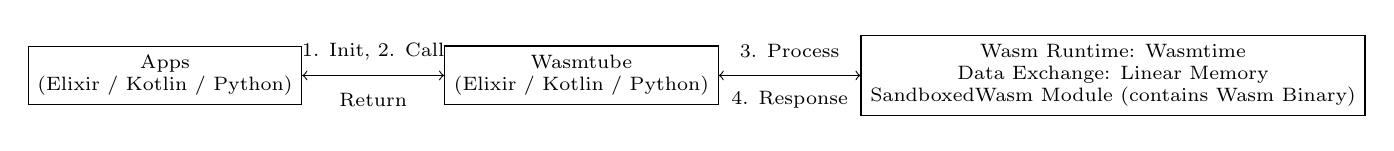
\begin{tikzpicture}[
    node distance=1.8cm,
    every node/.style={draw, minimum width=2cm, minimum height=0.6cm, align=center, font=\scriptsize}
]

% Nodes
\node (apps) {Apps \\ (Elixir / Kotlin / Python)};
\node (wasmtube) [right=of apps] {Wasmtube \\ (Elixir / Kotlin / Python)};
\node (runtime) [right=of wasmtube] {Wasm Runtime: Wasmtime \\ Data Exchange: Linear Memory \\ SandboxedWasm Module (contains Wasm Binary)};

% Arrows with labels
\draw[->] (apps) -- node[above, font=\scriptsize, draw=none]
    {1. Init, 2. Call} (wasmtube);

\draw[->] (wasmtube) -- node[above, font=\scriptsize, draw=none]
    {3. Process} (runtime);

\draw[->] (runtime) -- node[below, font=\scriptsize, draw=none]
    {4. Response} (wasmtube);

\draw[->] (wasmtube) -- node[below, font=\scriptsize, draw=none]
    {Return} (apps);

\end{tikzpicture}
\caption{Wasmtube Architecture: Multi-Language Support}
\end{figure}


\subsubsection{Multi-Language Support}

The Wasmtube concept demonstrates the universal nature of WebAssembly bridges. While the current implementation is Elixir-specific, the same architectural pattern can be implemented in other languages:

\begin{itemize}
\item \textbf{Kotlin/Java:} Using Wasmtime Java bindings or JNI wrappers
\item \textbf{Python:} Using wasmtime-py or similar Python bindings
\item \textbf{C/C++:} Direct integration with Wasmtime C API
\item \textbf{JavaScript/Node.js:} Using WebAssembly API
\end{itemize}

This multi-language support is what enables the isomorphic nature of IoT systems, where the same Wasm binary can run across different platforms and programming languages.

\subsection{Isomorphic IoT Systems}

The second solution enables the use of the same Wasm binary across different layers of IoT infrastructure, built from a common codebase. This approach provides:

\begin{table}[h]
\centering
\small
\begin{tabular}{|p{2.5cm}|p{2.5cm}|p{2.5cm}|p{2.5cm}|}
\hline
\multicolumn{4}{|c|}{\textbf{Wasm Runtime}} \\
\hline
\rowcolor{gray!30}
\textbf{Wasmtube} & \textbf{Wasmtube} & \textbf{Wasmtube} & \textbf{Wasmtube} \\
\hline
Node.js, Python & C/C++, Rust & Swift, Java, Kotlin, Flutter & C/C++, Rust, Elixir \\
\hline
Linux & Linux & iOS, Android OS & FreeRTOS, Linux \\
\hline
VM/Containers & RPi/Baremetal & iPhone, Android & ESP32, Raspberry Pi \\
\hline
Cloud & Edge/Gateway & Mobile & IoT Device \\
\hline
\end{tabular}
\caption{Isomorphic IoT Systems Architecture Across Different Platforms}
\end{table}


\begin{itemize}
\item \textbf{Code Reuse:} Same Wasm binary runs on different architectures (ARM, x86/64, arm64)
\item \textbf{Reduced Complexity:} Single codebase instead of multiple platform-specific versions
\item \textbf{Consistent Behavior:} Identical logic across device, edge, and cloud layers
\item \textbf{Simplified Deployment:} Single binary deployment process for all platforms
\end{itemize}

\section{Implementation and Technologies}

\subsection{Core Technologies}

\textbf{WebAssembly (Wasm)} \cite{webassembly2023}
\begin{itemize}
\item Binary format for stack-based virtual machines
\item Originally developed for web browsers
\item Platform-agnostic execution environment
\item Sandboxed security model with linear memory
\end{itemize}

\textbf{Apache TVM} \cite{apachetvm2023}
\begin{itemize}
\item Machine learning compiler framework
\item Compiles ML models to various target formats
\item Supports WebAssembly compilation
\item Enables deployment of ML models as Wasm binaries
\end{itemize}

\textbf{Elixir and Nerves Platform} \cite{nerves2023}
\begin{itemize}
\item Elixir: Functional programming language built on Erlang VM
\item Nerves: IoT development platform for Elixir
\item Provides reliable, fault-tolerant IoT device development
\item Handles system interfaces and hardware access
\end{itemize}

\subsection{Use Case Implementation}

The research demonstrates the concepts through a practical machine learning use case:

\begin{enumerate}[label=\arabic*.]
\item \textbf{Model Compilation:} ResNet-50 and MobileNetV2 models compiled to Wasm binaries using Apache TVM
\item \textbf{Cross-Platform Deployment:} Identical binaries deployed on Raspberry Pi 4, Google Cloud instances, and local machines
\item \textbf{Inference Processing:} Image recognition and classification using the same Wasm binary across all layers
\end{enumerate}

\section{Performance Evaluation}

\subsection{Overhead Analysis}

The study measured the overhead introduced by Wasm function calls:

\begin{itemize}
\item \textbf{Native Elixir execution:} 31.01 $\mu$s average
\item \textbf{Wasm function call:} 252.48 $\mu$s average
\item \textbf{Overhead:} $\sim$221 $\mu$s (approximately 200 $\mu$s as reported)
\end{itemize}

\subsection{Performance Results}

The overhead is acceptable because:

\begin{enumerate}[label=\arabic*.]
\item \textbf{Constant Overhead:} The 200$\mu$s overhead is nearly constant regardless of function complexity
\item \textbf{Negligible Impact:} For complex operations like ML inference, overhead becomes negligible (0.037\% for MobileNetV2)
\item \textbf{Practical Performance:} MobileNetV2 runs in approximately 0.6 seconds on Raspberry Pi 4
\end{enumerate}

\section{Design Tradeoffs}

\subsection{Performance vs. Flexibility}

\textbf{Trade-off:} Wasm introduces overhead but enables dynamic updates and cross-platform deployment.

\textbf{Justification:} The 200$\mu$s overhead is negligible for complex IoT operations while providing significant architectural benefits.

\subsection{Portability vs. Hardware Acceleration}

\textbf{Trade-off:} Wasm provides portability but currently lacks direct hardware acceleration support.

\textbf{Current State:} CPU-only execution limits performance for large models like ResNet-50 on resource-constrained devices.

\textbf{Future Prospects:} The wasi-nn specification development may enable GPU acceleration in the future.

\section{Security and Privacy Considerations}

\subsection{Security Benefits}

\begin{itemize}
\item \textbf{Sandboxed Execution:} Wasm provides an isolated execution environment
\item \textbf{Memory Safety:} Linear memory model prevents buffer overflows
\item \textbf{Code Integrity:} Wasm binaries can be verified before execution
\item \textbf{Controlled Access:} No direct system access, controlled by host application
\end{itemize}

\subsection{Security Challenges}

\begin{itemize}
\item \textbf{Core Application Security:} Core application still handles sensitive system operations
\item \textbf{Binary Distribution:} Need for secure channels for Wasm binary distribution
\item \textbf{Runtime Security:} Security depends on Wasm runtime implementation
\item \textbf{Malicious Binaries:} Potential for malicious Wasm binaries if not properly verified
\end{itemize}

\section{Outcomes and Future Directions}

\subsection{Current Success}

The study demonstrates significant practical benefits:

\begin{itemize}
\item \textbf{7x faster update times} compared to traditional firmware updates
\item \textbf{Successful cross-platform deployment} of ML models
\item \textbf{Practical performance} with MobileNetV2 achieving 0.6s inference on Raspberry Pi 4
\item \textbf{Reduced development complexity} through code reuse
\end{itemize}

\subsection{Future Research Directions}

\begin{enumerate}[label=\arabic*.]
\item \textbf{MLOps Integration:} Construction of MLOps flows using isomorphic IoT systems
\item \textbf{Workload-Aware Offloading:} Processing offloading across layers using common codebase
\item \textbf{Federated Learning:} Application to federated learning scenarios
\item \textbf{Hardware Acceleration:} Integration with wasi-nn for GPU acceleration
\end{enumerate}

\section{Conclusion}

This case study demonstrates that WebAssembly-based IoT systems offer a promising solution to critical challenges in modern IoT development. The research successfully addresses the need for rapid device updates and multi-platform development while maintaining practical performance characteristics.

The proposed dynamic IoT applications and isomorphic IoT systems provide significant benefits in terms of development efficiency, maintainability, and deployment flexibility. While current limitations exist regarding hardware acceleration, the foundation is established for future improvements that could further enhance the effectiveness of these approaches.

The study's success in addressing real-world IoT development challenges while maintaining practical performance characteristics makes it a valuable contribution to the field and a model for future research in IoT system architecture.

\bibliographystyle{ieeetr}
\bibliography{references}

\end{document}
